\documentclass[aspectratio=169,12pt]{beamer}
%\usepackage{forest}
\usepackage[T1]{fontenc}
%\usepackage{lmodern}

\usepackage[spanish, es-nodecimaldot]{babel}
%\usepackage{icomma} % Use dot as decimal separator
\usepackage{booktabs} % For better-looking tables
\usepackage{wrapfig}
\usepackage{caption}
%\usepackage{siunitx}


\usepackage{refcount}

\usepackage{multicol}
\usepackage{mathtools}

\usepackage[normalem]{ulem}

\pagestyle{empty}

\usepackage{pgf,tikz}
\usepackage{pgfplots}
\usetikzlibrary{matrix}
\usetikzlibrary{arrows}

%\usepackage{wrapfig}
\mode<presentation>
\usefonttheme{professionalfonts}
\usetheme{Darmstadt}
\usecolortheme{orchid}
\useoutertheme{default}
\setbeamertemplate{headline}{}

\renewcommand{\baselinestretch}{1.1}

%gets rid of bottom navigation bars
\setbeamertemplate{footline}[page number]

%gets rid of navigation symbols
\setbeamertemplate{navigation symbols}{}

%\frameframe{none} % No default frame

%\setlength{\framewidth}{8.7in} \setlength{\frameheight}{7.2in}

\parindent 0pt
\setlength{\parskip} {1ex plus 0.5ex minus 0.2ex}


%\usepackage[bbgreekl]{mathbbol}
\usepackage{amsfonts}

%\DeclareSymbolFontAlphabet{\mathbb}{AMSb}
%\DeclareSymbolFontAlphabet{\mathbbl}{bbold}

\newcommand{\Sym}{{\mathcal S}}
\DeclareMathOperator{\Aut}{Aut}
\DeclareMathOperator{\Tr}{Tr}
\DeclareMathOperator{\trace}{Trace}
\DeclareMathOperator{\range}{range}
\DeclareMathOperator{\rank}{rank}

\usepackage{breqn}
\usepackage{multicol}
\usepackage{colortbl}
\usepackage{lmodern}
\usepackage{tabularx}
\usepackage{multirow}
\usepackage{amssymb}
\usepackage{amsmath}
\usepackage{stmaryrd}
\usepackage{color}
\usepackage{graphicx}
\graphicspath{ {img/} }
\usepackage{hyperref}

\input{epsf}
\title{Introducción}
\author{}

\DeclareMathOperator{\Hom}{Hom}
\DeclareMathOperator{\sing}{sing}

\DeclareMathOperator{\chara}{char}
\DeclareMathOperator{\Jacob}{Jacob}
\DeclareMathOperator{\Sing}{Sing}
\newcommand{\fracNoLine}[2]{\genfrac{}{}{}{0pt}{#1}{#2}}

%\beamerdefaultoverlayspecification{<+->}

\usepackage{listings,xcolor,bm}


\definecolor{mygreen}{rgb}{0,0.6,0}
\definecolor{mygray}{rgb}{0.5,0.5,0.5}
\definecolor{mymauve}{rgb}{0.58,0,0.82}
\lstset{
  backgroundcolor=\color{white},   % choose the background color; you must add
  basicstyle=\small\ttfamily,      % the size of the fonts that are used for the code
  breakatwhitespace=false,         % sets if automatic breaks should only happen at whitespace
  breaklines=true,                 % sets automatic line breaking
  captionpos=b,                    % sets the caption-position to bottom
  commentstyle=\color{mygreen},    % comment style
  deletekeywords={...},            % if you want to delete keywords from the given language
  escapeinside={\%*}{*)},          % if you want to add LaTeX within your code
  extendedchars=true,              % lets you use non-ASCII characters; for 8-bits encodings only, does not work with UTF-8
  firstnumber=1,                % start line enumeration with line 1000
  frame=single,	                   % adds a frame around the code
  keepspaces=true,                 % keeps spaces in text, useful for keeping indentation of code (possibly needs columns=flexible)
  keywordstyle=\color{blue},       % keyword style
  language=Python,                 % the language of the code
  morekeywords={*,...},            % if you want to add more keywords to the set
  numbers=left,                    % where to put the line-numbers; possible values are (none, left, right)
  numbersep=5pt,                   % how far the line-numbers are from the code
  numberstyle=\tiny\color{mygray}, % the style that is used for the line-numbers
  rulecolor=\color{black},         % if not set, the frame-color may be changed on line-breaks within not-black text (e.g. comments (green here))
  showspaces=false,                % show spaces everywhere adding particular underscores; it overrides 'showstringspaces'
  showstringspaces=false,          % underline spaces within strings only
  showtabs=false,                  % show tabs within strings adding particular underscores
  stepnumber=5,                    % the step between two line-numbers. If it's 1, each line will be numbered
  stringstyle=\color{mymauve},     % string literal style
  tabsize=4,	                   % sets default tabsize to 2 spaces
  title=\lstname                   % show the filename of files included with \lstinputlisting; also try caption instead of title
}

\begin{document}

\newtheorem{prop}{Proposici\'on}
\newtheorem{algo}[prop]{Algorithm}
\newtheorem{teor}[prop]{Theorem}
\newtheorem{lema}[prop]{Lemma}
\newtheorem{coro}[prop]{Corollary}
\newtheorem{defi}[prop]{Definition}

\newcommand{\ideal}[1]{{\left\langle{#1}\right\rangle}}
\newcommand{\demo}{\textbf {Demostraci\'on. }}
\newcommand{\obse}{\textbf {Observaci\'on. }}
\newcommand{\Input}{\textbf {Input: }}
\newcommand{\Output}{\textbf {Output: }}
\newcommand{\Examp}{\textbf {Ejemplo }}
\newcommand{\Examps}{\textbf {Ejemplos }}

\newcommand{\kk}{{\mathbbl k}}
\newcommand{\V}{{\mathbf V}}
\newcommand{\I}{{\mathbf I}}
\newcommand{\PP}{{\tilde P}}
\newcommand{\QQ}{{\tilde Q}}

\newcommand{\F}{{\mathbb F}}
\newcommand{\Q}{{\mathbb Q}}
\newcommand{\N}{{\mathbb N}}
\newcommand{\R}{{\mathbb R}}
\newcommand{\Z}{{\mathbb Z}}
\newcommand{\CC}{{\mathbb C}}
\newcommand{\eLL}{{\mathcal L}}



\newcommand{\MinAss}{\textrm {MinAss}}
\newcommand{\Ass}{\textrm {Ass}}
\newcommand{\mcm}{\textrm {mcm}}
\newcommand{\mcd}{\textrm {mcd}}
%\newcommand{\mod}{\textrm { mod }}
\newcommand{\lt}{\textrm {lt}}
\newcommand{\Lt}{\textrm {Lt}}
\newcommand{\lp}{\textrm {lp}}
\newcommand{\lc}{\textrm {lc}}
\newcommand{\lm}{\textrm {lm}}
\newcommand{\barra}{\ /\ }
\newcommand{\multideg}{\textrm {multideg}}

\newcommand{\sep}{\textrm {sep}}
\newcommand{\Syz}{\textrm {Syz}}
\newcommand{\n}{\~n}
\newcommand{\cG}{\textrm {cG}}
\newcommand{\dG}{\textrm {dG}}
\newcommand{\nG}{\textrm {nG}}
\newcommand{\CE}{\textrm {CE}}
\newcommand{\CG}{\textrm {CG}}
\newcommand{\CF}{\textrm {CF}}
\newcommand{\DG}{\textrm {DG}}
\renewcommand{\NG}{\textrm {NG}}

\newcommand{\p}{{\boldsymbol{p}}}
\newcommand{\q}{{\boldsymbol{q}}}

\newcommand{\X}{{\boldsymbol{X}}}
\newcommand{\x}{{\boldsymbol{x}}}
\renewcommand{\u}{{\boldsymbol{u}}}
\renewcommand{\t}{{\boldsymbol{t}}}
\renewcommand{\a}{{\boldsymbol{a}}}
\renewcommand{\b}{{\boldsymbol{b}}}
\renewcommand{\c}{{\boldsymbol{c}}}

%Titulos en espa�ol
%\renewcommand{\chaptername}{Cap\'{\i}tulo}
%\renewcommand{\bibname}{Bibliograf\'{\i}a}

\newcommand{\kring}{\kk[\x]}
\newcommand{\kRing}{\kk[X]}
\newcommand{\qring}{\Q[\x]}

%\renewcommand\itemindent{-10pt}
%\renewcommand{\theenumi}{\arabic{enumi}}
%\renewcommand{\labelenumi}{\Alph{enumi}}

\definecolor{issac}{rgb}{1.00,0.00,0.00}
%------------------------------------------------------------------

\begin{frame}

 \begin{center}

\Large\textbf{Laboratorio de Datos} \\
\large\textbf{Clustering: $k$-medias}
%\vspace{0.5cm}

% \textit{Santiago Laplagne} \\
%slaplagn@dm.uba.ar \\


\vspace{1cm}
Primer Cuatrimestre 2024 \\ Turnos tarde y noche

\vspace{1cm}


 {\small Facultad de Ciencias Exactas y Naturales, UBA}
 \end{center}


\end{frame}

%------------------------------------------------------------------


\begin{frame}
\frametitle{Introducción a las Técnicas de Clasificación}
\begin{itemize}
    \item \textbf{Definición:} La clasificación es una técnica de aprendizaje supervisado donde el objetivo es predecir la categoría a la que pertenece una nueva observación, basada en un conjunto de datos de entrenamiento con categorías conocidas.
    \item \textbf{Aplicaciones Comunes:}
    \begin{itemize}
        \item Diagnóstico médico (clasificación de enfermedades)
        \item Reconocimiento de imágenes (clasificación de objetos)
        \item Filtrado de correos electrónicos (spam vs no spam)
    \end{itemize}
\end{itemize}
\end{frame}

\begin{frame}
\frametitle{Técnicas Comunes de Clasificación}
\begin{itemize}
    \item \textbf{Regresión Logística:}
    \begin{itemize}
        \item Método estadístico para modelar la probabilidad de una variable binaria
        \item Utiliza una función logística para limitar los valores predichos entre 0 y 1
    \end{itemize}
    \item \textbf{K-Vecinos Más Cercanos (K-NN):}
    \begin{itemize}
        \item Clasifica basándose en la mayoría de los vecinos más cercanos a un punto de datos
        \item Sencillo pero puede ser computacionalmente costoso
    \end{itemize}
\end{itemize}
\end{frame}

\begin{frame}
\frametitle{Otras Técnicas de Clasificación}
\begin{itemize}
    \item \textbf{Árboles de Decisión:}
    \begin{itemize}
        \item Modelo basado en reglas de decisión en forma de árbol
        \item Fácil de interpretar y visualizar
    \end{itemize}
    \item \textbf{Máquinas de Vectores de Soporte (SVM):}
    \begin{itemize}
        \item Encuentra el hiperplano que maximiza el margen entre las diferentes clases
        \item Eficaz en espacios de alta dimensión
    \end{itemize}
    \item \textbf{Redes Neuronales:}
    \begin{itemize}
        \item Modelos inspirados en el funcionamiento del cerebro humano
        \item Capaces de aprender representaciones complejas
    \end{itemize}
\end{itemize}
\end{frame}

\begin{frame}
\frametitle{Árboles de decisión: ejemplo}

\begin{tikzpicture}[edge from parent/.style={draw, -latex}, sibling distance=10em, level distance=4em]
\tikzset{
        level 1/.style={level distance=15mm,sibling distance=80mm},
        level 2/.style={level distance=15mm,sibling distance=30mm},
        level 3/.style={level distance=15mm,sibling distance=30mm},
        level 4/.style={level distance=15mm,sibling distance=30mm},
    }
  \node {¿Salario $\ge 1.000.000$?}
    child { node {Sí}
      child { node {¿Bienes totales $\ge 10.000.000$?}
        child { node {Sí}
          child { node {Dar crédito} }
        }
        child { node {No}
          child { node {No dar crédito} }
        }
      }
    }
    child { node {No}
      child { node {¿Bienes totales $\ge 20.000.000$?}
        child { node {Sí}
          child { node {Dar crédito} }
        }
        child { node {No}
          child { node {No dar crédito} }
        }
      }
    };
\end{tikzpicture}
\end{frame}

\begin{frame}
\frametitle{Support vector machine: ejemplo}

\begin{minipage}[t]{.4\textwidth}
\textbf{Caso lineal}

Separamos los puntos por rectas o planos.

\begin{center}
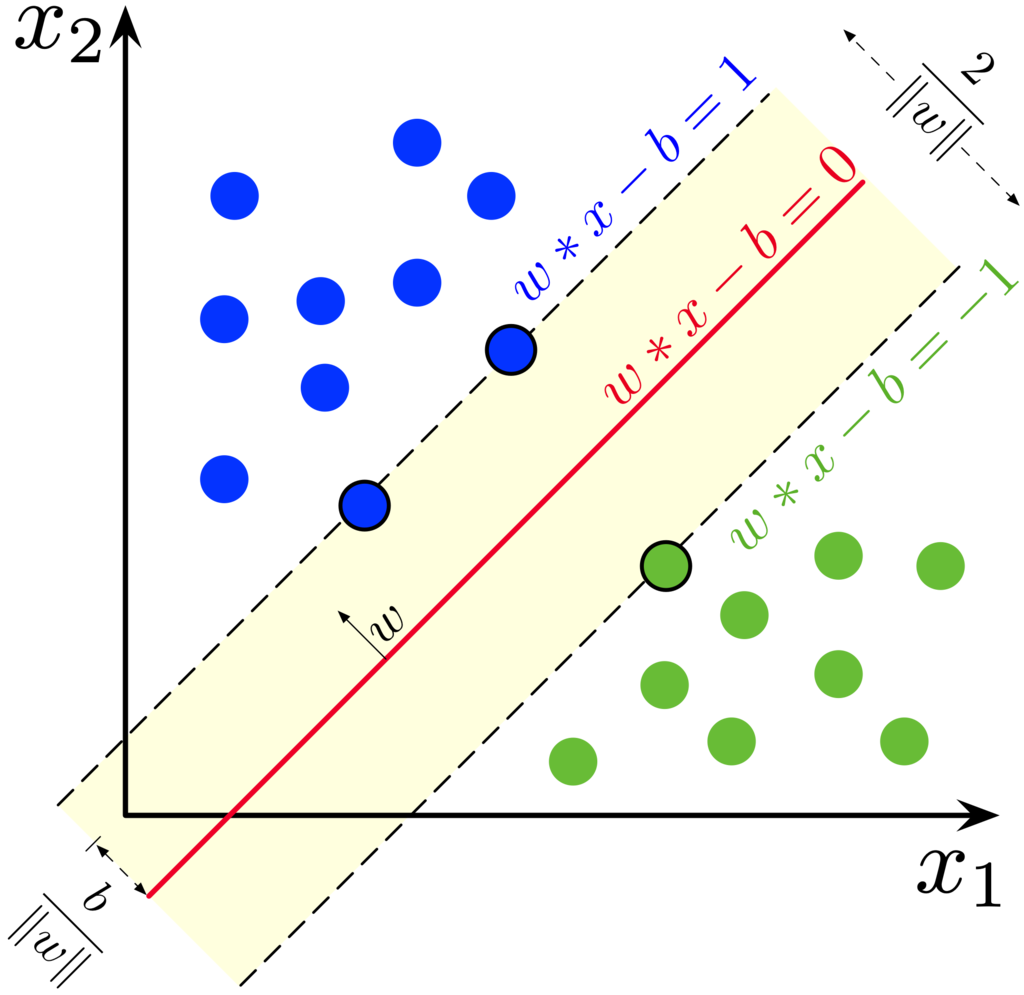
\includegraphics[scale=0.4]{clase17_SVM_margin_lineal.png}
\end{center}

\end{minipage} \hspace{.4cm} %
\begin{minipage}[t]{.4\textwidth}
\textbf{Caso no lineal}

Antes de separar por un plano, aplicamos una transformación de los datos.

\begin{center}
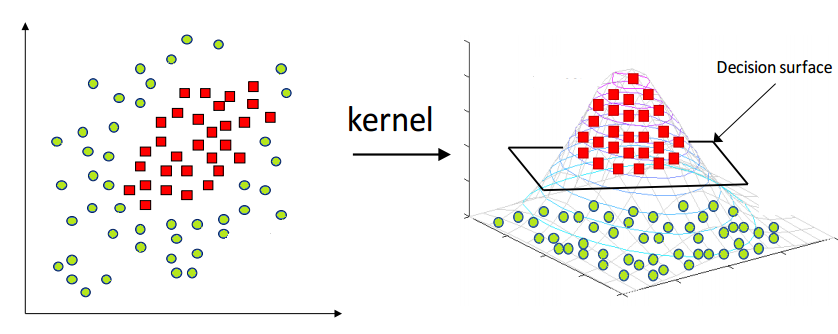
\includegraphics[scale=0.22]{clase17_SVM_margin_nolineal.png}
\end{center}

\end{minipage}


\end{frame}

\begin{frame}
\frametitle{Regresión Logística en 1 minuto}

\begin{minipage}{.5\textwidth}
¿Cómo podemos predecir una variable respuesta binaria ($0/1$)?

Considerar a $y$ como una variable numérica y ajustar una función lineal $y = \beta_0 + \beta_1 x$ no va a ser apropiado.

\vspace{1cm}

Queremos una función que para valores grandes positivos de $x$ la función se acerque a 1 y para valores grandes negativos la función se acerque a 0.

\end{minipage}%
\begin{minipage}{.5\textwidth}
    \begin{center}
    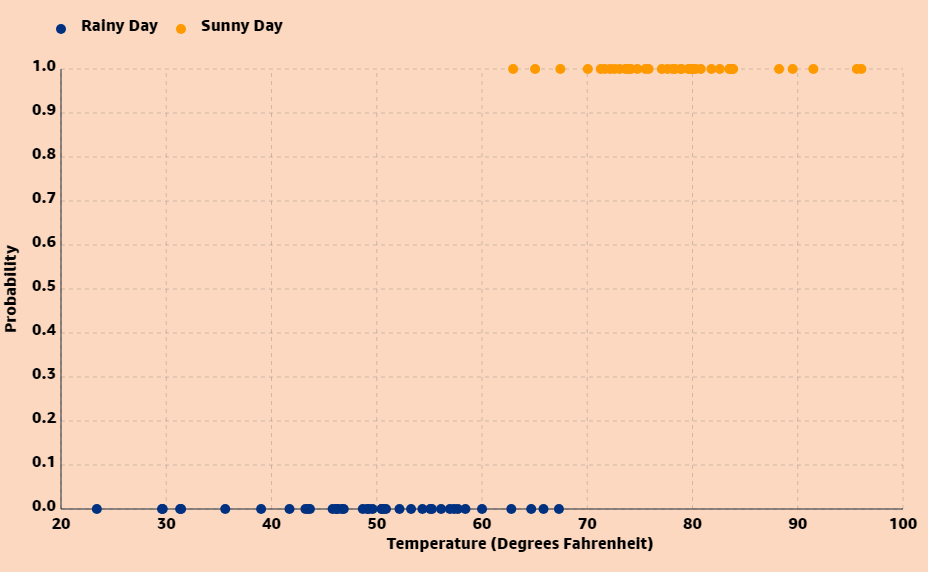
\includegraphics[scale=0.24]{clase17-variable_binaria.png}
    \end{center}
\end{minipage}

\end{frame}

\begin{frame}
\frametitle{Regresión Logística en 1 minuto}

\begin{minipage}{.5\textwidth}

Le aplicamos una transformación a la función lineal. 

En regresión logística tomamos
$$
y = \frac{1}{1 + e^{-(\beta_0 + \beta_1 x)}}.
$$

Si $\beta_1$\textgreater$0$, cuanto mas grande es $x$, más cercano a 1 es $y$.

\vspace{.5cm}

Si tenemos varias variables explicativas, usamos
$$
y = \frac{1}{1 + e^{-(\beta_0 + \beta_1 x_1 + \beta_2 x_2 + \dots + \beta_n x_n)}}.
$$


\end{minipage}%
\begin{minipage}{.5\textwidth}
    \begin{center}
    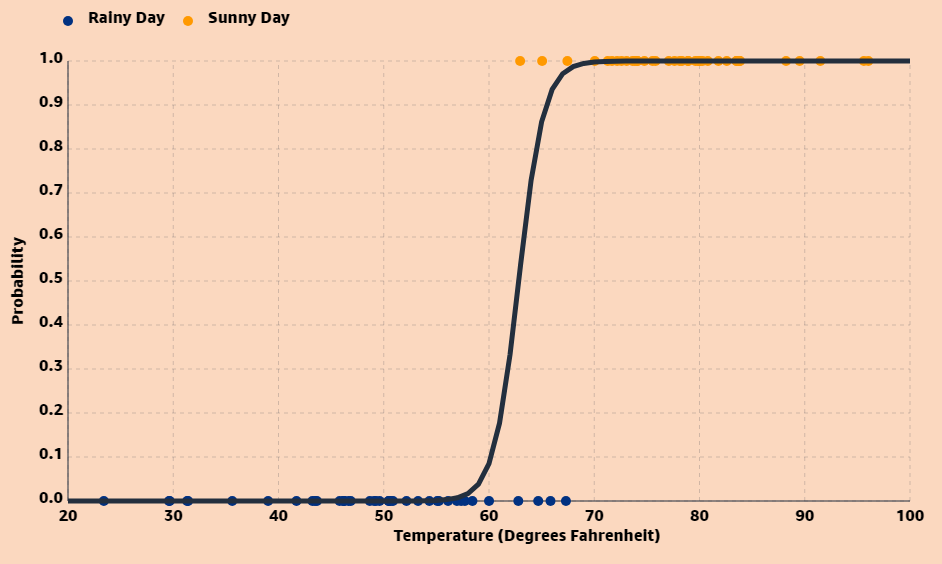
\includegraphics[scale=0.24]{clase17-variable_binaria_logit.png}
    \end{center}
\end{minipage}

\end{frame}

\begin{frame}
\frametitle{Regresión Logística en 1 minuto}

\begin{minipage}{.5\textwidth}

Finalmente usamos la curva para clasificar.

$$
y = \frac{1}{1 + e^{-(\beta_0 + \beta_1 x)}}.
$$

\end{minipage}%
\begin{minipage}{.5\textwidth}
    \begin{center}
    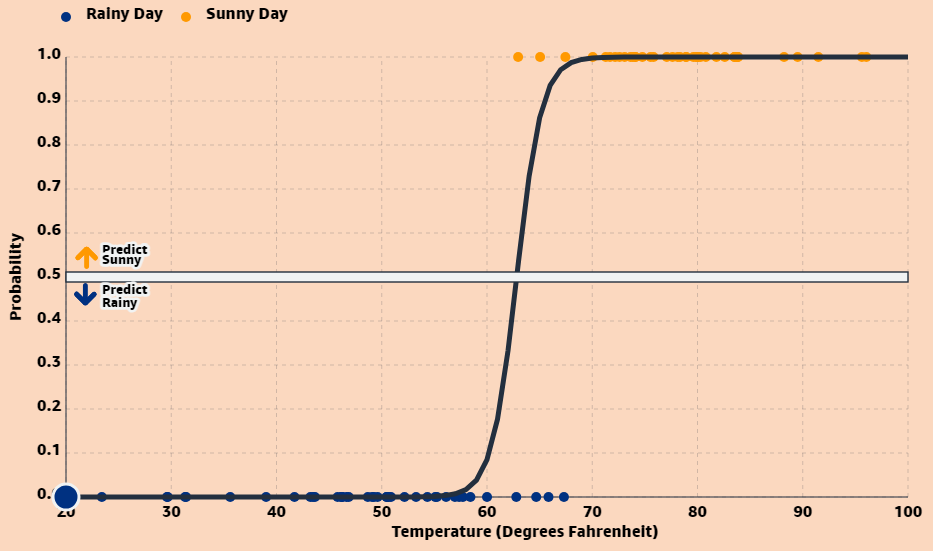
\includegraphics[scale=0.24]{clase17-variable_binaria_predict.png}
    \end{center}
\end{minipage}
\end{frame}


\begin{frame}
\frametitle{Métodos paramétricos vs. no paramétricos}

\begin{itemize}
\item Los modelos de regresión lineal o regresión logística son modelos paramétricos.
\item Asumen una forma específica para la relación entre las variables independientes y la variable dependiente.
\item Es decir, se define una ecuación paramétrica con un número fijo de parámetros (coeficientes) que determinan esta relación, por ejemplo $y = \frac{1}{1 + e^{-(\beta_0 + \beta_1 x)}}$.
\item Los métodos paramétricos hacen suposiciones sobre la distribución de los datos y la estructura del modelo, lo que puede proporcionar predicciones más eficientes y precisas si estas suposiciones son correctas.
\end{itemize}

¿Cómo sería un método no-paramétrico?
\end{frame}

\begin{frame}
\frametitle{Modelo no paramétrico para clasificación}

Tenemos un conjunto de pingüinos para los que sabemos su especie, y queremos saber la especie de un nuevo pingüino.

¿A qué especie pertenece el pingüino rojo?

\begin{center}
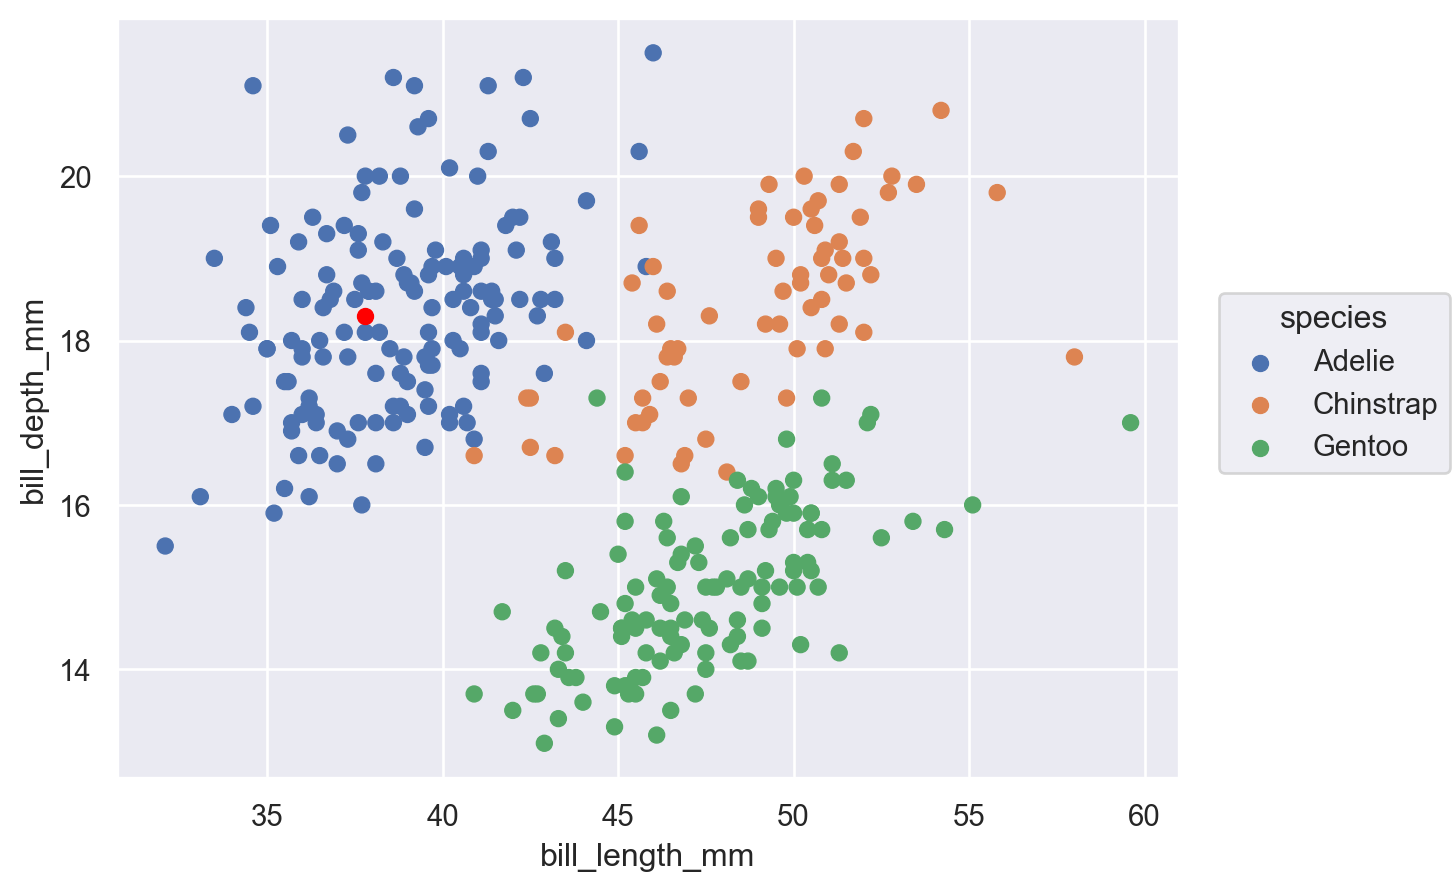
\includegraphics[scale=0.24]{clase17-pinguino1.png}
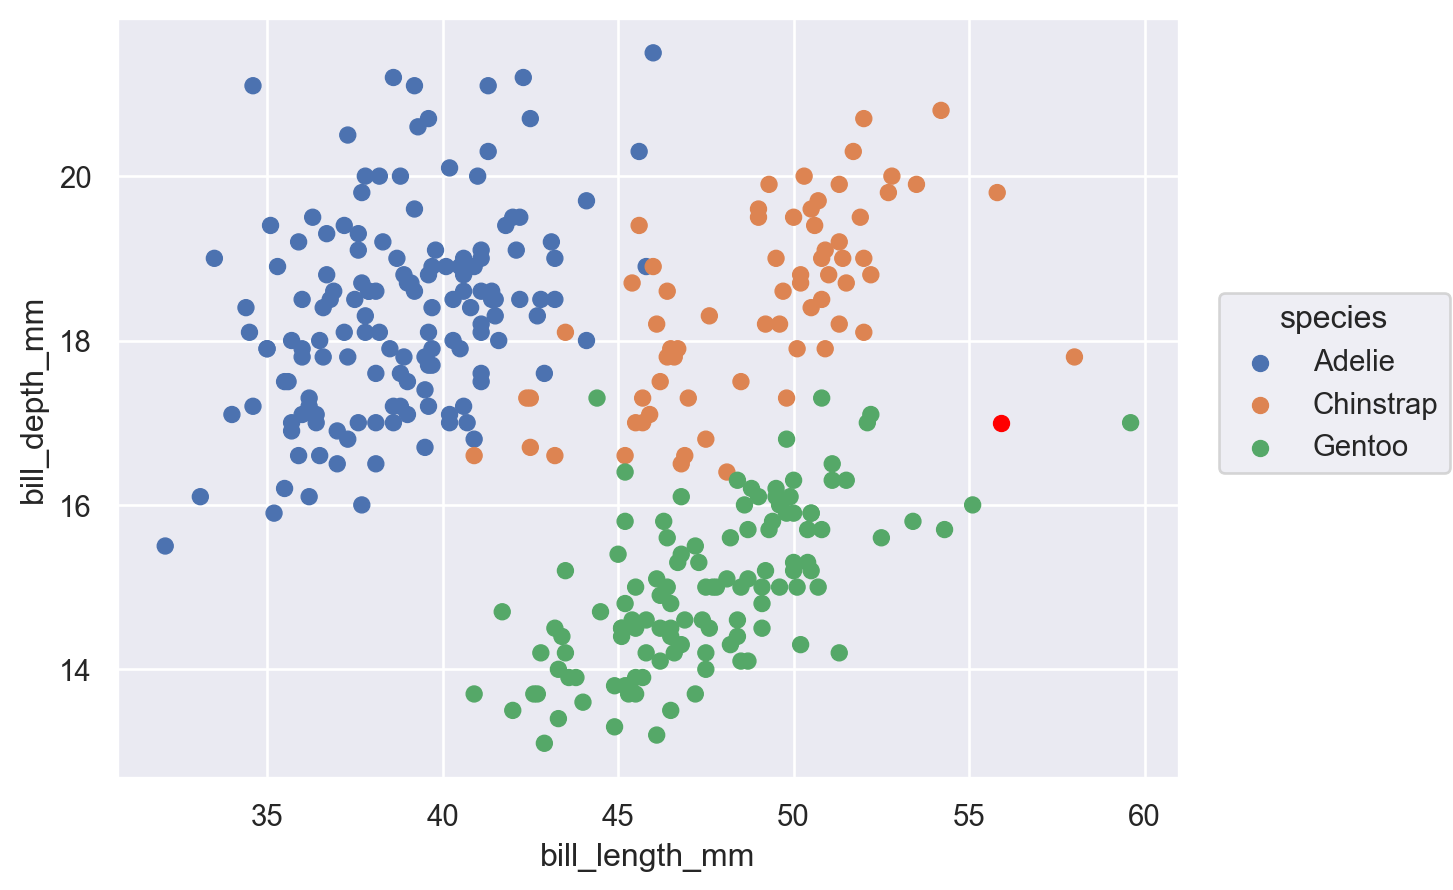
\includegraphics[scale=0.24]{clase17-pinguino2.png}
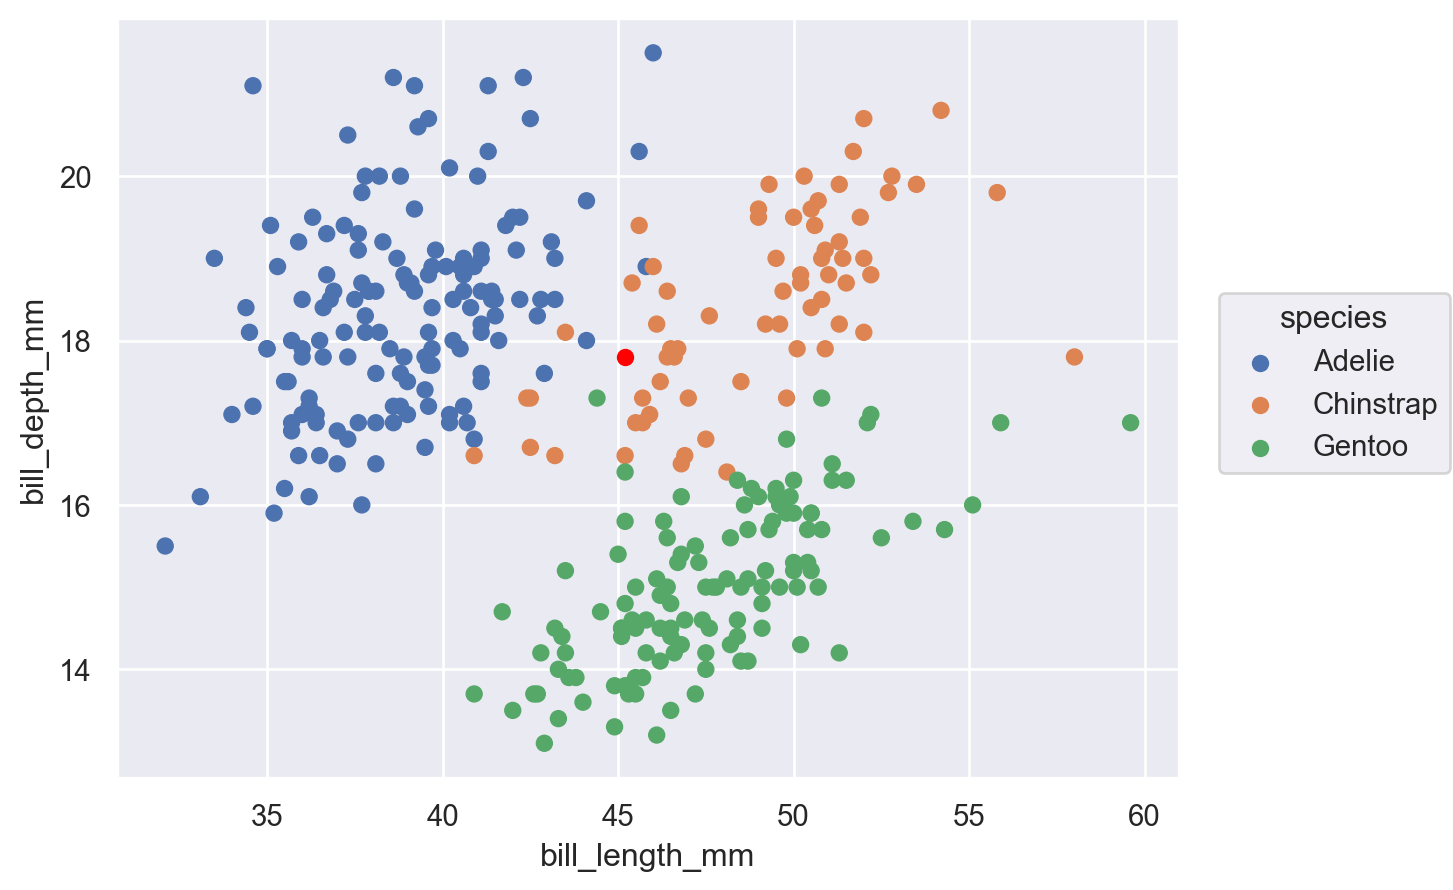
\includegraphics[scale=0.24]{clase17-pinguino3.png}
\end{center}

\end{frame}

\begin{frame}
\frametitle{¿Qué es el Algoritmo K-Vecinos Más Cercanos (K-NN)?}
\begin{itemize}
    \item \textbf{Definición:}
    \begin{itemize}
        \item K-NN es un algoritmo de aprendizaje supervisado utilizado para clasificación y regresión.
        \item Se basa en la idea de que objetos similares están cerca unos de otros.
    \end{itemize}
    \item \textbf{Funcionamiento:}
    \begin{itemize}
        \item Para clasificar un nuevo punto, el algoritmo busca los $K$ puntos más cercanos en el conjunto de entrenamiento.
        \item La categoría más común entre estos $K$ vecinos se asigna al nuevo punto.
    \end{itemize}
\end{itemize}
\end{frame}

\begin{frame}
\frametitle{Características y Aplicaciones del Algoritmo K-NN}
\begin{itemize}
    \item \textbf{Ventajas:}
    \begin{itemize}
        \item Fácil de entender e implementar.
        \item No requiere un modelo paramétrico, lo que lo hace flexible.
    \end{itemize}
    \item \textbf{Desventajas:}
    \begin{itemize}
        \item Computacionalmente costoso para grandes conjuntos de datos debido a la necesidad de calcular distancias.
        \item El rendimiento puede verse afectado por la elección del valor de K y la escala de las características.
        \item Si tenemos muchas variables explicativas, sufriremos la maldición de la dimensionalidad.
    \end{itemize}
\end{itemize}
\end{frame}

%------------------------------------------------------------------

\begin{frame}
\frametitle{Selección del $K$-óptimo}

Como es un modelo de aprendizaje supervisado, podemos elegir el $K$ óptimo con alguna estrategia de validación.

Esquema posible de validación:

\begin{enumerate}
\item Separamos el conjunto de todos los datos en 80\% entrenamiento y 20\% testeo
\item Elegimos el valor de $K$ por validación cruzada en la muestra de entrenamiento.
\item Probamos la perfomance de nuestro modelo en la muestra testeo.
\end{enumerate}

Preguntas:
\begin{itemize}
\item ¿Cuál es el valor a optimizar en la validación? Elegimos el valor de $K$ que nos de el mayor porcentaje de aciertos.
\item ¿Qué significa entrenar nuestro modelo? Como es un modelo no-paramétrico, no hay que aprender ningún parámetro. Entrenar es simplemente guardar los datos.
\end{itemize}

\end{frame}

\begin{frame}
\frametitle{Validación "leave-one-out"}

Podemos hacer validación cruzada en pliegos:

\begin{itemize}
\item Dividimos nuestra muestra en 5 pliegos (o cualquier otra cantidad).
\item Seleccionamos 4 pliegos para entrenamiento y 1 pliego para validación.
\item Para cada uno de los datos de validación, buscamos los $K$ vecinos más cercanos en los pliegos de entrenamiento.
\item Elegimos el valor más votado entre los vecinos.
\end{itemize}

Validación leave-one-out.
\begin{itemize}
\item Es el caso extremo de validación en pliegos, donde cada observación es un pliego.
\item Para cada observación, buscamos los $K$ vecinos más cercanos entre todos los demás puntos.
\item Elegimos el valor más votado entre los vecinos.
\end{itemize}

En modelos de regresión, validación leave-one-out puede ser costoso porque debemos entrenar nuevamente el modelo para cada observación. En KNN, como no hay que ajustar parámetros, este método no tiene costo adicional comparado con usar pocos pliegos.

\end{frame}

\end{document}

%------------------------------------------------------------------

\begin{frame}[fragile]
\frametitle{Aplicación de K-means en Python}
\begin{itemize}
    \item Ejemplo de implementación en Python usando \texttt{scikit-learn}:
\end{itemize}

\begin{lstlisting}
from sklearn.cluster import KMeans
import numpy as np

# Datos de ejemplo
X = np.array([[1, 2], [1, 4], [1, 0],
              [10, 2], [10, 4], [10, 0]])

# Inicializar K-means
kmeans = KMeans(n_clusters=2, random_state=0).fit(X)

# Resultados
print(kmeans.labels_)
print(kmeans.cluster_centers_)
\end{lstlisting}

\end{frame}
